\documentclass{article}
\usepackage{graphicx}
\usepackage{pdflscape}
\usepackage{pdfpages}
\begin{document}

\title{CS3810 Business Plan}

\author{Daniel Atkinson (daa9)}
%\date{March 14, 2013}
\maketitle

\newpage
\tableofcontents
\newpage

\section{Business Description}
Anti-Entropy is company specialising in mobile applications for back office sales systems.  The currently supported platforms are the iOS and Android operating systems.  The aim of this product is to give busineses a simple solution to managing information on customers, provided products and services.  This application may even replace dedicated terminals with a more convenient form factor, idealy installed on company supplied phones or tablets.
\\We also provide server hardware which hosts a central database the mobile software interacts with for its operations.  This can either be renting our hosting service or purchasing a dedicated server for installation on the customers premesis.
\\To use the software the customer must pay a monthly licence fee, there are available per device or at a larger cost, per company.  When purchasing a product the customer gets their first month licence for free.
\\Packaged with the licence we offer support services to help streamline the integration of our products into a customers business.

\section{Competitor Analysis}
The main competitors for this type of product would be similar products and the dedicated hardware versions as well as companies that offer similar back end sales management.
\\Companies that offer sich services are:
\begin{itemize}
\item ACT!
\\A CRM solution software package created by Sage.
\\This seems to be a Windows only solution with no Mac, Linux or mobile support apart from some standard calendar syncing features.
\\They also offer a support package at a cost.

\item Goldmine
\\It has a mobile version as well as a desktop version with integration into Microsoft Outlook.
\\The mobile version is only available on iOS and requires a windows server to host the service.
\\This solution also seems to have third party plugin support for a few additional features.

\item Maximizer
\\Maximizer CRM Which also has iCalendar integration as well as a web based access tot he system.
\\It has mobile versions as well including blackberry and windows mobile (not windows phone).

\end{itemize}



\section{Strengths}
We have solutions for the two main current mobile platforms as well as offering both hosted and dedicated database options.
\\Providing a personal service by having a friendly sales team who get to know each of our customers businesses directly and offer to meet on their own premesis.

\section{Weaknesses}
The costs of starting up and generating an initial income is the greatest weakness during the early stages of the business.
\\Competitors are already established and can already generate revenue to stay afloat.
\\\\The second weakness would be awareness, the competitors are already known or easily found.  Getting the brand out to potential customers and portraying our product as a quility brand.

\section{Opportunities}
The internet is a very cheap and effective medium for gaining awareness and for easy communication between us as a company and our customers.
\\Anti-Entropy will focus on good business to business relationships to try and establish brand loyalty and to help tailor our service to their individual needs.
\\A lot of these services are just a software package with optional support with no need to talk to a human being, just order the software and you are done, we offer a personal service to help integrate with existing businesses.

\section{Threats}
Already established products are much more likely to get the sales over a new unknown product.
\\If the venture is very successfull then there is the possibility of work overload where we may not be able to deliver all of the services promtly and to the standard of which the customer is expecting.

\section{Personnel}
\begin{itemize}
\item Managing Director
\\Will be responisble to the top level management of the business and making sure that all of the finances are managed appropriately.

\item Senior Developer
\\Responsible for the development team.  Should have a Computer Science or programming background.

\item Web Developer
\\Creation an maintenance of the company website will be the responsibility of the web developer, which should expand to a team when the company is more established.  Also will work on the web client for the product.

\item Developer
\\Standard developer working on the product itself.  Idealy having one developer per application (iOS, Android, Server).  Initialy developers will have to provide support for their products as well.

\item HR Manager
\\Will be tasked with making sure the Government criteria for workplaces is met and that staff are kept happy.  Primarily ensuring a productive workforce.

\item Sales
\\Responsible for contacting other businesses about our product and building relationships with them, as well as aquiring sales.

\item Marketing Manager
\\To seek our potential customers to give to sales, to organise and manage advertising.  Should be familiar with digital marketing.
\end{itemize}



\section{Marketing}
Co-ordination between the sales team and the marketing manager will be key to successfull marketing.
\begin{itemize}
\item Traditional advertising
\\In business magazines and newspapers.

\item Targeted adverts on websites.

\end{itemize}

\section{Justifications}
To keep the utility costs down we should rent office space which has utilities included including a T1 broadband internet line.
\\Sales staff will use their personal vehicles or public transport, depending on distance needed to travel, untill the company is established enough and can afford the expense of company vehicles.
\\\\The reasons behind choosing iOS and Android as the mobile platforms for this venture is due to the increasing market share of these devices over the alternatives.  According to Tech-Thoughts \cite{tech} Android has had an increasing market share over iOS and currently has much more of the market than its competitor.  iOS is the next highest and is on the rise.
\begin{figure}[h]
\centering
        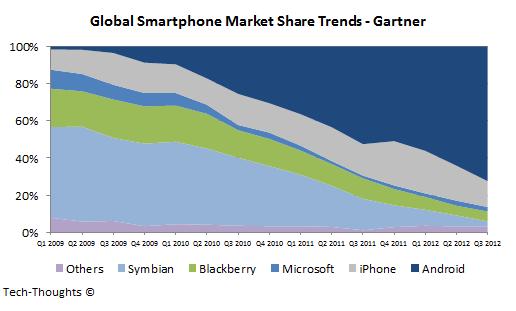
\includegraphics{market_share.png}
        \caption{Smartphone market share}
        \label{Smartphone market share}
\end{figure}




\begin{landscape}
\begin{figure}[h]
\centering
        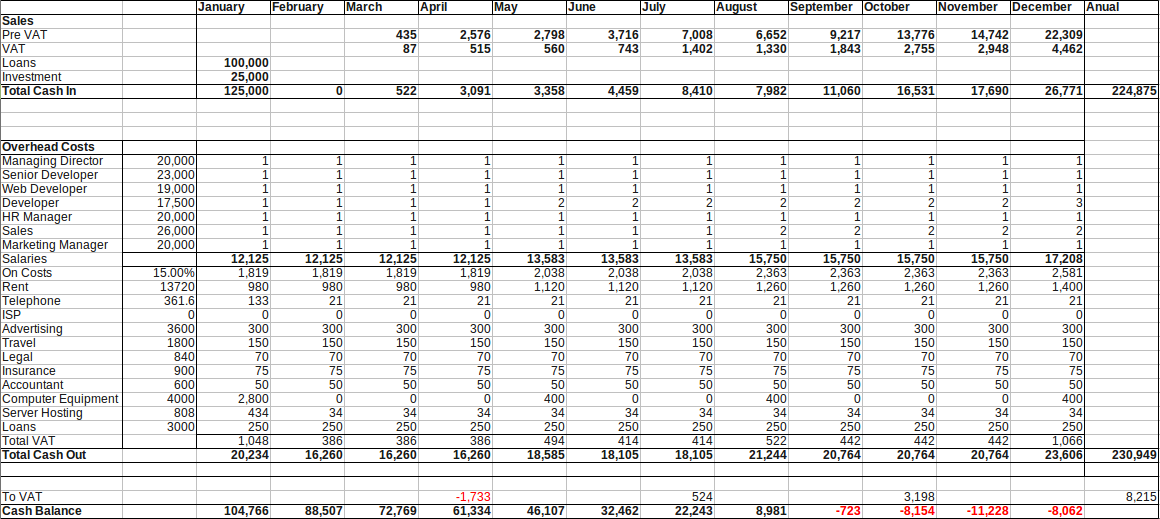
\includegraphics[width=9.0in]{cash_flow_year1.png}
        \caption{1st Year Cash Flow}
        \label{1st Year Cash Flow}
\end{figure}

\begin{figure}[h]
\centering
        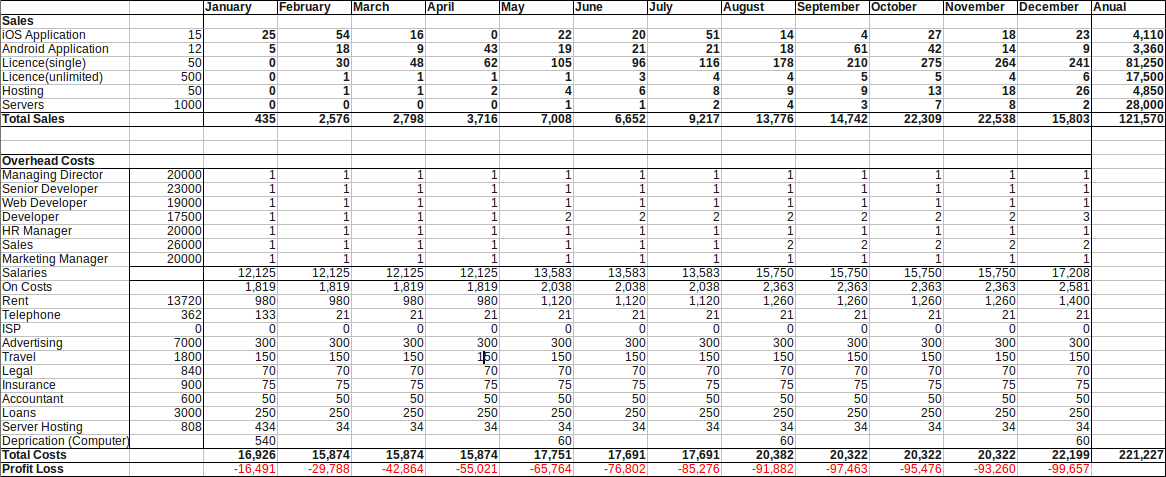
\includegraphics[width=9.0in]{profit_loss_year1.png}
        \caption{1st Year Profit/Loss}
        \label{1st Year Profit/Loss}
\end{figure}

\end{landscape}

\begin{figure}[h]
\centering
        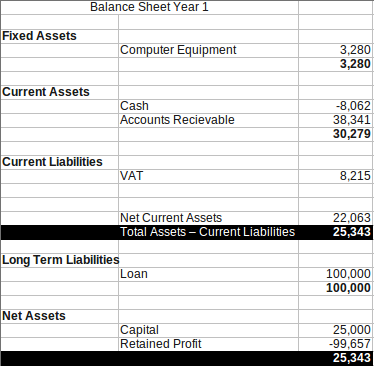
\includegraphics[width=3.0in]{balance_sheet_year1.png}
        \caption{1st Year Balance Sheet}
        \label{1st Year Balance Sheet}
\end{figure}

\begin{landscape}

\begin{figure}[h]
\centering
        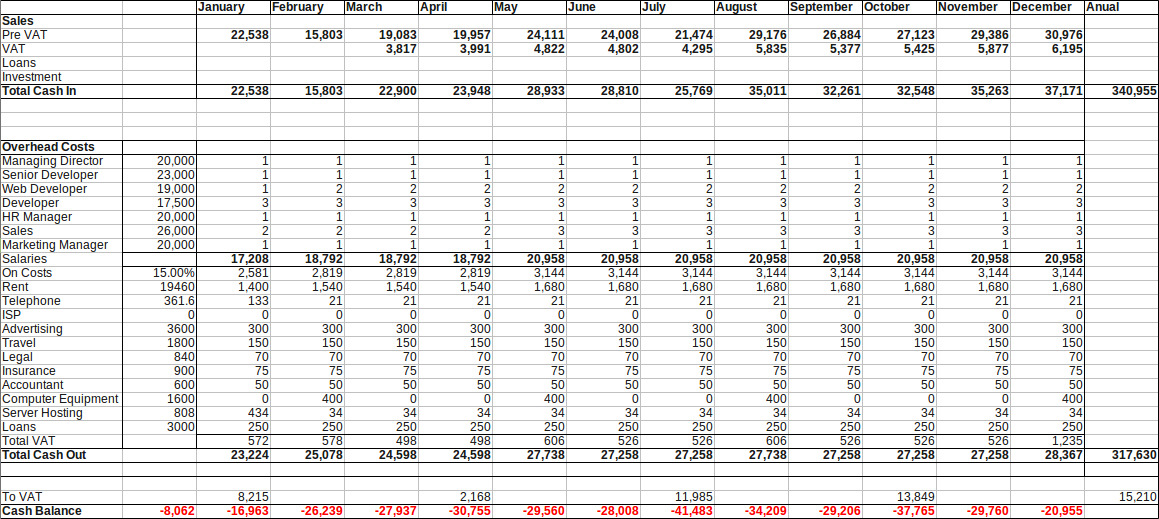
\includegraphics[width=9.0in]{cash_flow_year2.png}
        \caption{2nd Year Cash Flow}
        \label{2nd Year Cash Flow}
\end{figure}

\begin{figure}[h]
\centering
        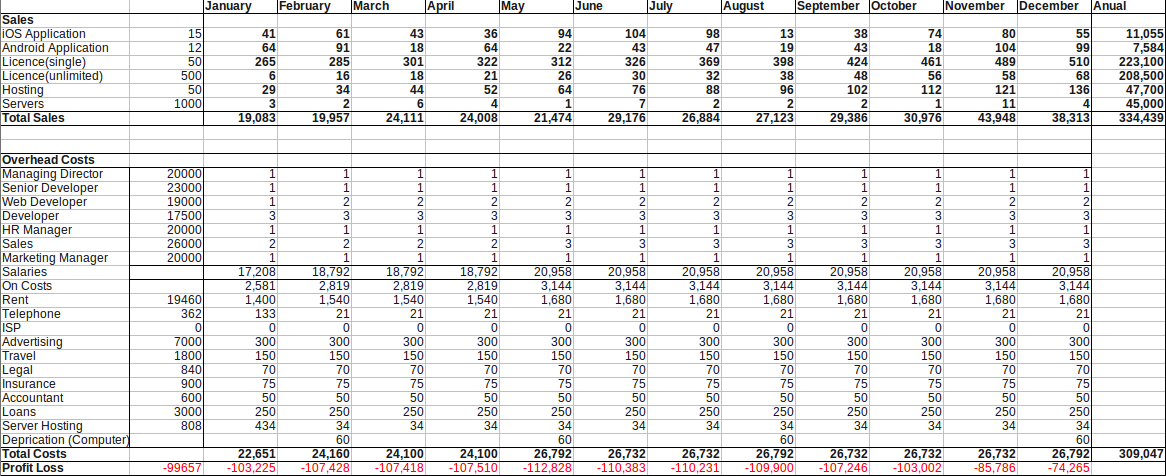
\includegraphics[width=9.0in]{profit_loss_year2.png}
        \caption{2nd Year Profit/Loss}
        \label{2nd Year Profit/Loss}
\end{figure}

\end{landscape}
\begin{figure}[h]
\centering
        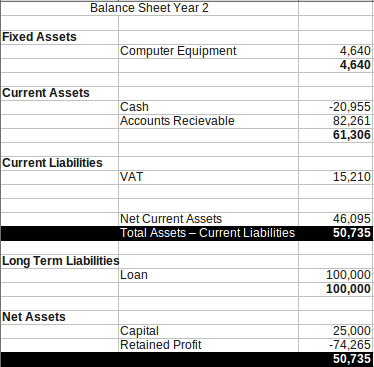
\includegraphics[width=3.0in]{balance_sheet_year2.png}
        \caption{2nd Year Balance Sheet}
        \label{2nd Year Balance Sheet}
\end{figure}


\begin{thebibliography}{9}
\bibitem{reed} UK job site, http://www.reed.co.uk, accessed 16/03/2013
\\Used to research average saleries for various job types.

\bibitem{act!} Sage CRM software, http://shop.sage.co.uk, accessed 15/03/2013
\\Research ACT!, Sage CRM software.

\bibitem{Goldmine} Goldmine, http://www.goldmine.com, accessed 15/03/2013
\\Research Goldmine CRM software.

\bibitem{Maximizer} Maximizer CRM, http://www.max.co.uk, accessed 15/03/2013
\\Research Maximizer CRM software.

\bibitem{instantoffice} Flexible office specialists, http://instantoffices.com, accessed 17/03/2013
\\Price of office space rental

\bibitem{BT} BT business phone, http://business.bt.com, accessed 17/03/2013
\\Reference for business phone line pricing

\bibitem{rapidswitch} Dedicated Server Hosting, http://rapidswitch.com, accessed 17/03/2013
\\Pricing for dedicated server hosting

\bibitem{accounting} Cheap accounting from qualified accountants, http://www.cheapaccounting.co.uk, accessed 18/03/2013
\\Reference for some budget accounting services

\bibitem{tech} Smartphone market share, http://www.tech-thoughts.net/2012/12/smartphone-market-share-trends-by-country.html, accessed 18/03/2013
\\Researching device market share

\end{thebibliography}

\end{document}
